\section{Aplicación al modelo binomial}
Usemos toda la información obtenida para llegar a una fórmula que nos permitirá establecer el precio de una opción europea. Para ello, utilizaremos un modelo binomial con más de un paso en el que suponemos que $ d = 1 $. De este modo, tenemos un activo sin riesgo con precios $ S^0 $ y uno con riesgo con precios $ S^1$ los cuales denotaremos por $ S $. También, como mencionamos anteriormente, sin pérdida de generalidad asumimos que $ S^0_0  = 1$ por lo que $ S_t^0 =  (1+r)^t $ para $ t \in \mathbb{T} $. Los precios de nuestro activo con riesgo vienen determinados por $ S_{t-1}(1+u) $ o $ S_{t-1}(1+d) $ cumpliendo $ -1 < d < u $, es decir, siguen una distribución de Bernoulli. El valor inicial $ S_0 $ es constante y conocido. Tomamos entonces como espacio de probabilidad $ \Omega = \{1+u,1+d\}^T $ con la filtración $ \mathbb{F} $ dada por $ \mathcal{F}_0 = \{\emptyset, \Omega\} $ y $ \mathcal{F}_t = \sigma(S_u^1: \hspace{1mm} u \leq t) $ para $ t >0 $. Para $ \omega = \{\omega_1,\dots,\omega_n\} $ en $ \Omega $ definimos
\[
P(\{\omega\}) = P(\frac{S_t}{S_{t-1}} = \omega_t, \hspace{1mm} t=1,\dots,T).
\]
Notamos a $ \frac{S_t}{S_{t-1}} $ como $ R_t $ tal y como ya hemos hecho anteriormente. Veamos la relación necesaria entre $ d,u \text{ y } r$ para que tengamos una medida martingala equivalente.
\bigskip
\begin{lemaBox}\label{cotasUpDown}
	Para tener una EMM en el modelo binomial se debe cumplir que $ d < r < u $.
\end{lemaBox}
\begin{proof}
	Sea $ Q $ una probabilidad en $ (\Omega, \mathcal{F}) $. Para que sea una martingala equivalente se debe dar:
	\[
	E_Q(\bar{S}_t | \mathcal{F}_{t-1}) = \bar{S}_{t-1}.
	\]
	\[
	\big\Updownarrow
	\]
	\[
	E_Q(R_t | \mathcal{F}_{t-1} ) = E_Q(\frac{\bar{S}_t}{\bar{S}_{t-1}} | \mathcal{F}_{t-1}) = E_Q(\frac{\beta_t}{\beta_{t-1}} | \mathcal{F}_{t-1}) = \frac{\beta_t}{\beta_{t-1}} = 1+r.
	\]
	Como $ R_t $ solo puede tomar valores $ 1+u $ y $ 1+d $, su valor medio solo puede $ 1+r $ si, y solo si, $ d < r < u $.
\end{proof}
\bigskip

A continuación, vamos a construir dicha medida $ Q $ mediante el siguiente lema:
\bigskip
\begin{lemaBox}
	El proceso $ \bar{S} $ es una $ (\mathbb{F},Q) $-martingala si, y solo si, las variables aleatorias $ R_t $ son independientes e idénticamente distribuidas con $ Q(R_1 = 1+u) = \frac{r-d}{u-d}$ y $ Q(R_1 = 1+d) = 1- \frac{r-d}{u-d} $. Además, si el modelo es viable, $ Q $ es única.
\end{lemaBox} 
\begin{proof}
	Para simplificar la notación, llamamos $ q =  \frac{r-d}{u-d}$.
	\begin{itemize}
		\item[$ \Longleftarrow $)] Como $ R_t $ son independientes:
		\[
		E_Q(R_t | \mathcal{F}_{t-1}) = E_Q(R_t) = q(1+u) + (1-q)(1+d) = q(u-d) + 1 +d = 1+r.
		\]
		Siguiendo un proceso similar a la demostración del lema \ref{cotasUpDown}, vemos que efectivamente es una $ (\mathbb{F},Q) $-martingala.
		\item[$ \Longrightarrow $)] En este caso, $ E_Q(R_t | \mathcal{F}_{t-1}) = 1+r $. Como solo puede tomar valores $ 1+u $ y $ 1+d $, se debe cumplir que
		\[
		(1+d)Q(R_1 = 1+d | \mathcal{F}_{t-1}) + (1+u)Q(R_1 = 1+u | \mathcal{F}_{t-1}) = 1+r
		\]
		y
		\[
		Q(R_1 = 1+d | \mathcal{F}_{t-1}) + Q(R_1 = 1+u | \mathcal{F}_{t-1}) = 1.
		\]
		Llamando $ q =  Q(R_1 = 1+u | \mathcal{F}_{t-1})$ obtenemos
		\[
		(1+d)(1-q) + (1+u)q = 1+r \Longrightarrow q = \frac{r-d}{u-d}.
		\]
		Con un argumento inductivo, para $ \omega = (\omega_1,\dots,\omega_T) \in \Omega $ vemos que
		\[
		Q(R_1 = \omega_1,\dots,R_t = \omega_t) = \prod_{i=1}^{t}q_i
		\]
		donde
		\[
		q_i =  \begin{cases}
		q & \text{ si } \omega_i = 1+u\\
		1-q& \text{ si } \omega_i = 1+d
		\end{cases}.
		\]
		Por lo tanto, las variables $ R_t $ son independientes e idénticamente distribuidas.
	\end{itemize}
	
	Finalmente veamos la unicidad. Es claro que $ q \in (0,1) $ si, y solo si, $ d<r<u $. Por ello, usando el teorema \ref{VIABLEiofEMM} y el lema \ref{cotasUpDown}, obtenemos que el modelo admite una única EMM que además es $ Q $.
\end{proof}
\bigskip

Al valor $ q = (r-d)/(u-d) $ obtenido en el resultado anterior se le suele denominar \textit{probabilidad de riesgo neutral}. Es un objeto matemático abstracto que no tiene que coincidir con la probabilidad real del mercado o estar relacionada con la misma y que de hecho, se conoce \textit{a priori}. Sin embargo, para la valoración de opciones se utiliza $ q $ ya que es la que hace que los precios actualizados se comporten según una martingala tal y como acabamos de probar. De este modo, la ganancia $ C_T = \left[S_T - K\right]^+$ de una opción \textit{call} en el instante $ t \in \mathbb{T} $ viene dada por
\[
V_t(C_T) = \frac{1}{\beta_t} E_Q(\beta_T C_T | \mathcal{F}_t).
\]
Usando la definición de $ R_t $, vemos que se cumple la siguiente relación:
\[
S_T = S_t \prod_{u = t+1}^{T}R_u.
\]
Podemos calcular su media ya que $ S_t $ es $ \mathcal{F}_t $-medible y $ R_u $ son independientes de $ \mathcal{F}_t $ si $ u > t $. De ese modo,
\begin{equation*}
\begin{split}
V_t (C_T) &= \frac{\beta_T}{\beta_t}E_Q(\left[S_t\prod_{u=t+1}^{T}R_u - K\right]^+ | \mathcal{F}_t) \\
&= (1+r)^{t-T} E_Q(\left[S_t\prod_{u=t+1}^{T}R_u - K\right]^+| \mathcal{F}_t) \\
& = (1+r)^{t-T} \sum_{v=0}^{T-t}\binom{T-t}{v}q^v(1-q)^{T-t-v}\left[S_t(1+u)^v(1+d)^{T-t-v}-K\right]^+,
\end{split}
\end{equation*}
donde en el último paso se ha usado la fórmula \eqref{valorBino}. Finalmente, en el instante 0, el valor de la opción es:
\begin{equation*}
V_0(C_T) = (1+r)^{-T} \sum_{v=A}^{T}\binom{T}{v}q^v(1-q)^{T-v}\left[S_0(1+u)^v(1+d)^{T-v}-K\right],
\end{equation*}
donde $ A $ denota el primer entero $ k $ que cumple $ S_0(1+u)^k(1+d)^{T-k} > K $. Esto se debe a que \[\left[S_0(1+u)^j(1+d)^{T-j}-K\right]^+ = 0, \hspace{1mm}\text{ para } j<k.\]

Esta fórmula nos aporta el valor de una opción \textit{call} o de compra. En la explicación de estos activos derivados dijimos que también existían las denominadas opciones \textit{put} o de venta. Gracias a la ausencia de arbitraje podemos calcular el precio de una en función del precio de la otra. A este hecho se le denomina \textit{paridad put-call}. Si denominamos por $ C_t $ al precio de la opción \textit{call} y como $ P_t $ al de la opción \textit{put} y tenemos en cuenta las ganancias como muestran las gráficas \ref{graphCall} y \ref{graphPut}, se da la siguiente relación. 

\[
C_T - P_T = (S_T - K)^+ - (K-S_T)^+ = S_T - K.
\]
Esta relación se debe dar para todo $ t \in \mathbb{T} $ y si consideramos la actualización del valor de $ K $ en cada instante mediante el interés $ r $ llegamos a:
\[
C_t - P_t = S_t - (1+r)^{-(T-t)}K,
\]
donde el $ (1+r)^{-(T-t)} $ es el factor de actualización entre los instantes $ t $ y $ T $. Este hecho es bastante conocido y aparece recogido, por ejemplo, en \cite{elliot1999mathematics}.\\

Una vez obtenida la fórmula y hecha la aclaración sobre la relación de precios entre los dos tipos de opciones, podemos realizar una serie de simulaciones para ver cómo varía el precio de una opción de compra según los distintos parámetros $ (K, T, S, d, r, u) $. Estas simulaciones se han realizado en  \textit{SageMath 2.8}. Para ello se han implementado las siguientes funciones como se observa en \ref{definiciones}: una para obtener el valor de $ A $ llamada \textit{getA} y otro el de la propia opción, \textit{getV}.

\begin{lstlisting}[label={definiciones}, caption={Definición en Sage de las funciones}, morekeywords={sage}]
sage: def getA(K, T, S, d, u):
          k = 0
          while S*(1+u)^(k)*(1+d)^(T-k) < K:
                k+=1
          return k
sage: def getV(K, T, S, d, r, u):
          A = getA(K, T, S, d, u)
          q = (r-d)/(u-d)
          if r <= d or r >= u:
              return 0
          else:
              return (1+r)^(-T)*sum(binomial(T,v)*q^v*(1-q)^(T-v)*(S*(1+u)^(v)*(1+d)^(T-v)- K) for v in range(A,T))           	 
\end{lstlisting}

Para ello, partiremos del siguiente problema general del que iremos variando los diferentes parámetros en el que tomamos una unidad monetaria (u.m.) cualquiera. \\

\textit{``Las acciones de una empresa tienen valor actual 25 u.m. cada una. Queremos comprar acciones de dicha empresa pero no estamos seguros de obtener una gran ganancia con ellas en el futuro. Por eso, decidimos realizar una opción de compra de aquí a un año en el que se nos ofrece un precio de 27 u.m. Los tiempos se mueven en el intervalo de meses. Según las estimaciones suponemos que en cada mes el retorno podría ser de 1.2 (u = 0.2)  pero también podemos perder dinero llegando este a tomar el valor 0.72 (d = -0.28). Consideramos que el precio del dinero se incrementa de manera constante cada mes un 0.1 (de este modo el mercado es viable).''} \\

El precio en esta situación es aproximadamente de 12.9325 u.m. Veamos cómo varía en función de cada parámetro manteniendo el resto como en el enunciado. En primer lugar, consideremos el valor como función de $ T $ y tomamos valores desde un mes hasta dos años, es decir, 24 meses. Los resultado se obtienen en la figura \ref{valueT}. También se incluye un ejemplo del código en \ref{pintar} para dibujar la gráfica en este caso junto con la definición de los parámetros generales5. Para el resto de parámetros se hace de manera análoga. 

\begin{lstlisting}[label={pintar}, caption={Código en Sage para dibujar una gráfica}, morekeywords={sage}]
sage:K = 27
T = 12
S = 25
d = -0.28
r = 0.1
u = 0.2
sage: point([(T, getV(K, T, S, d, r, u)) for T in srange(1, 25,1) ], rgbcolor = (1,0,0), size = 35, axes_labels=['$T$','$V_0(C_T)$'])          	 
\end{lstlisting}

\begin{figure}[h!]
	%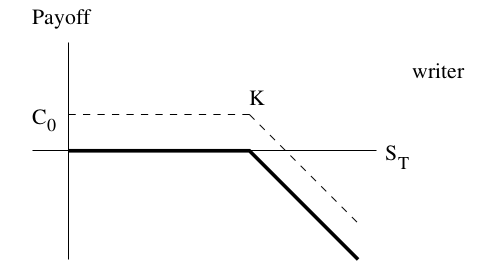
\includegraphics[width=1\linewidth]{Writer_call}
	\centering
	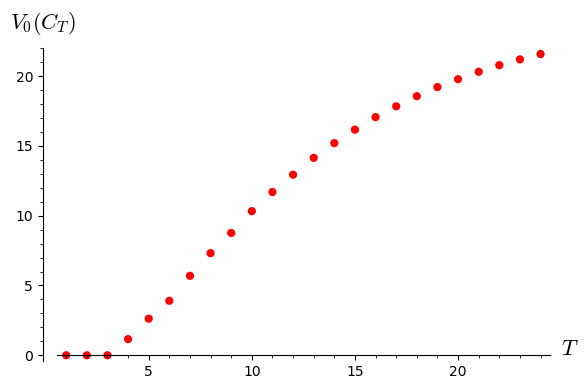
\includegraphics[width=0.6\linewidth]{value_T}
	\caption{Valor de la opción en función del número de pasos.}
	\label{valueT}
\end{figure}

Vemos que tendríamos que poner una fecha de compra superior a los 4 meses ya que durante los tres primeros $ A = T $, lo que significa que lo más seguro es que no ejerciéramos nuestro derecho a la opción. Observamos que los valores crecen en función de este parámetro. Veamos qué pasa si variamos el precio de la acción fijado en la opción de compra, es decir, $ K $. Se ha obtenido des este modo la gráfica \ref{valueK} en la que $ K $ varía de 23 a 33. Vemos que en este caso es decreciente. Esta situación podemos considerar que es la esperada. Cuanto menor sea precio más posibilidades tiene el propietario de ejercerla ya que es raro que en el futuro la acción tenga ese valor tan bajo. Por ello, el vendedor tiene que exigir un mayor. Por otro lado, cuanto mayor sea el precio acordado es el comprador el que corre un mayor riesgo de no ejercerla en el futuro por lo que tiene que pagar menos por ella ahora. 

\begin{figure}[h!]
	%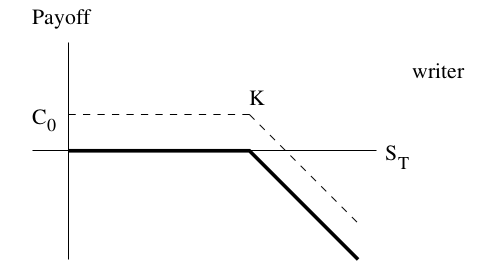
\includegraphics[width=1\linewidth]{Writer_call}
	\centering
	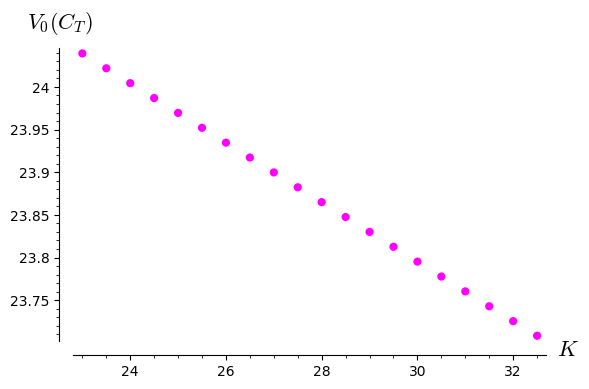
\includegraphics[width=0.6\linewidth]{value_K}
	\caption{Valor de la opción en función del precio acordado.}
	\label{valueK}
\end{figure} 

Obtengamos ahora el precio en función del valor actual $ S_0 $. Hemos variado dicho valor entre 23 y 33. Los resultados se muestras en la gráfica \ref{valueS}. 

\begin{figure}[h!]
	%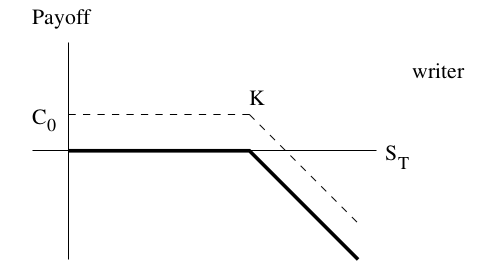
\includegraphics[width=1\linewidth]{Writer_call}
	\centering
	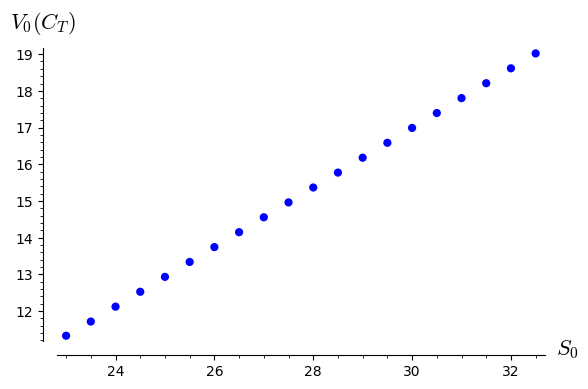
\includegraphics[width=0.6\linewidth]{value_S}
	\caption{Valor de la opción en función del valor actual.}
	\label{valueS}
\end{figure}
En este caso vuelven a ser crecientes, lo que era de esperar, ya que en la fórmula vemos que el precio de la opción es proporcional al valor actual de la misma. Finalmente, variemos los valores de  $ u, d \text{ y } r$ teniendo en cuenta las restricciones del lema \ref{cotasUpDown}. En la gráfica \ref{valuer} se muestran los resultados en función de $ r $.
\begin{figure}[h!]
	%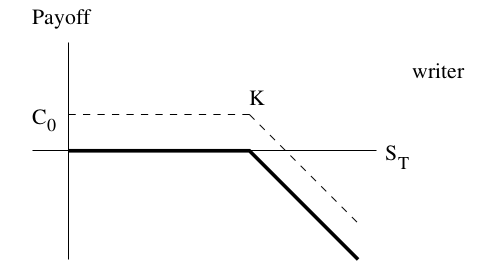
\includegraphics[width=1\linewidth]{Writer_call}
	\centering
	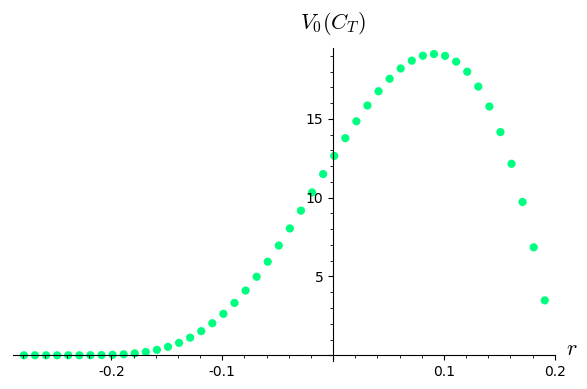
\includegraphics[width=0.6\linewidth]{value_r}
	\caption{Valor de la opción en función del interés.}
	\label{valuer}
\end{figure}
La variación de este valor es quizás la más interesante desde el punto de vista del vendedor de la opción. El parámetro $ r $ es en cierto modo subjetivo ya que es una estimación del valor que tendrá el dinero en el futuro. Por ello, según los valores fijados de $ d $ y $ u $ puede ver con qué interés obtiene el mayor beneficio. Es claro que si $ r < 0 $ significa que el dinero en el futuro tendrá menos valor y es una situación que en principio no la contemplamos ya que suponemos que el valor del dinero aumentará en un futuro. De todos modos, se han usado valores negativos para ver su evolución. Para $ r \geq 0 $ vemos que en este caso la función alcanza un máximo que como hemos dicho es el valor más favorable al vendedor. Si consideramos un interés mayor al mismo le estamos exigiendo demasiada rentabilidad y eso hace bajar el precio de la opción. Veamos cómo varía ahora para valores de $ u $ entre $ -0.4 $ y $ 0.1 $ mostrados en la gráfica \ref{valued}.
\begin{figure}[h!]
	%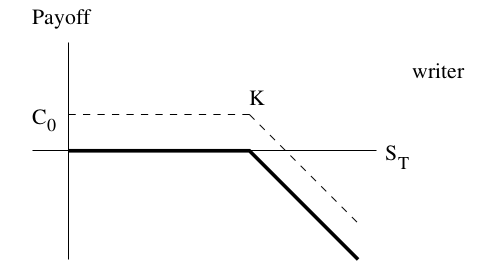
\includegraphics[width=1\linewidth]{Writer_call}
	\centering
	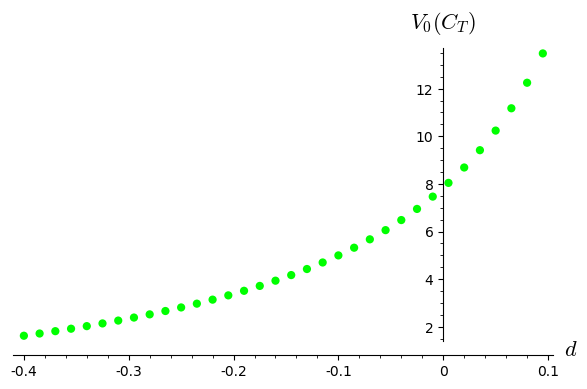
\includegraphics[width=0.6\linewidth]{value_d}
	\caption{Valor de la opción en función de $ d $.}
	\label{valued}
\end{figure}
En este caso también es creciente lo que es normal ya que cuanto mayor sea $ d $ mayor será la posible ganancia del comprador. Por último veamos cómo varía en función de $ u $. Para ello se han tomado valores entre $ 0.1 $ y $ 0.55 $. Se muestran en la gráfica \ref{valueu}.
\begin{figure}[h!]
	%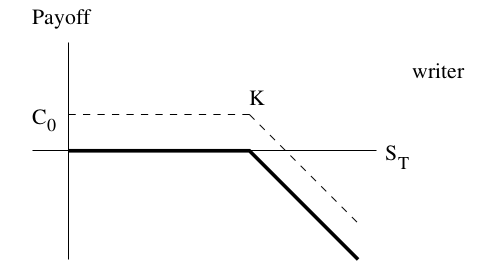
\includegraphics[width=1\linewidth]{Writer_call}
	\centering
	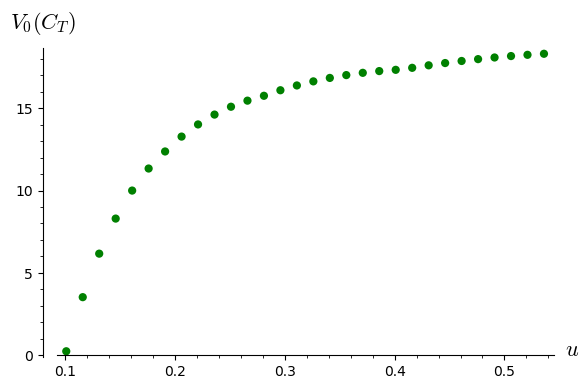
\includegraphics[width=0.6\linewidth]{value_u}
	\caption{Valor de la opción en función de $ u $.}
	\label{valueu}
\end{figure}

Observamos que para valores cercanos al interés el valor de la opción es relativamente bajo ya que la ganancia que obtendremos sería menor. El precio va aumentando aunque llega un punto que dicho crecimiento se reduce.